\documentclass{beamer}
%
% Choose how your presentation looks.
%
% For more themes, color themes and font themes, see:
% http://deic.uab.es/~iblanes/beamer_gallery/index_by_theme.html
%
\mode<presentation>
{
  \usetheme{default}      % or try Darmstadt, Madrid, Warsaw, ...
  \usecolortheme{crane} % or try albatross, beaver, crane, ...
  \usefonttheme{structurebold}  % or try serif, structurebold, ...
  \setbeamertemplate{navigation symbols}{}
  \setbeamertemplate{caption}[numbered]
} 

\usepackage[english]{babel}
\usepackage[utf8x]{inputenc}
\usepackage{listings}

\title[ML]{Machine Learning}
\author{Pawel Wocjan}
\institute{University of Central Florida}
\date{Spring 2019}

\begin{document}

\begin{frame}
  \titlepage
\end{frame}

\begin{frame}{Convolutional neural networks}
\begin{itemize}
\item A breakthrough in building models for image classification came with the discovery that a convolutional neural network (CNN) could be used to progressively extract higher and higher slevel representations of the image content. 
\item Instead of preprocessing the data to derive features like textures and shapes, a CNN takes just the image's raw pixel data as input and ``learns'' how to extract these features, and ultimately infer what object they constitute.
\end{itemize}
\end{frame}

\begin{frame}{CNN}
\begin{itemize}
\item To start, the CNN receives an input feature map: a three-dimensional matrix, where
\begin{itemize}
\item the size of the first two dimensions corresponds to the length and width of the images in pixels and
\item the size of the third dimension is 3 (corresponding to the 3 channels of a color image: red, green, and blue). 
\end{itemize}
\item The CNN comprises a stack of modules, each of which performs three operations.
\end{itemize}
\end{frame}

\begin{frame}{Illustration of end-to-end structure of a convolutional neural network}
\medskip
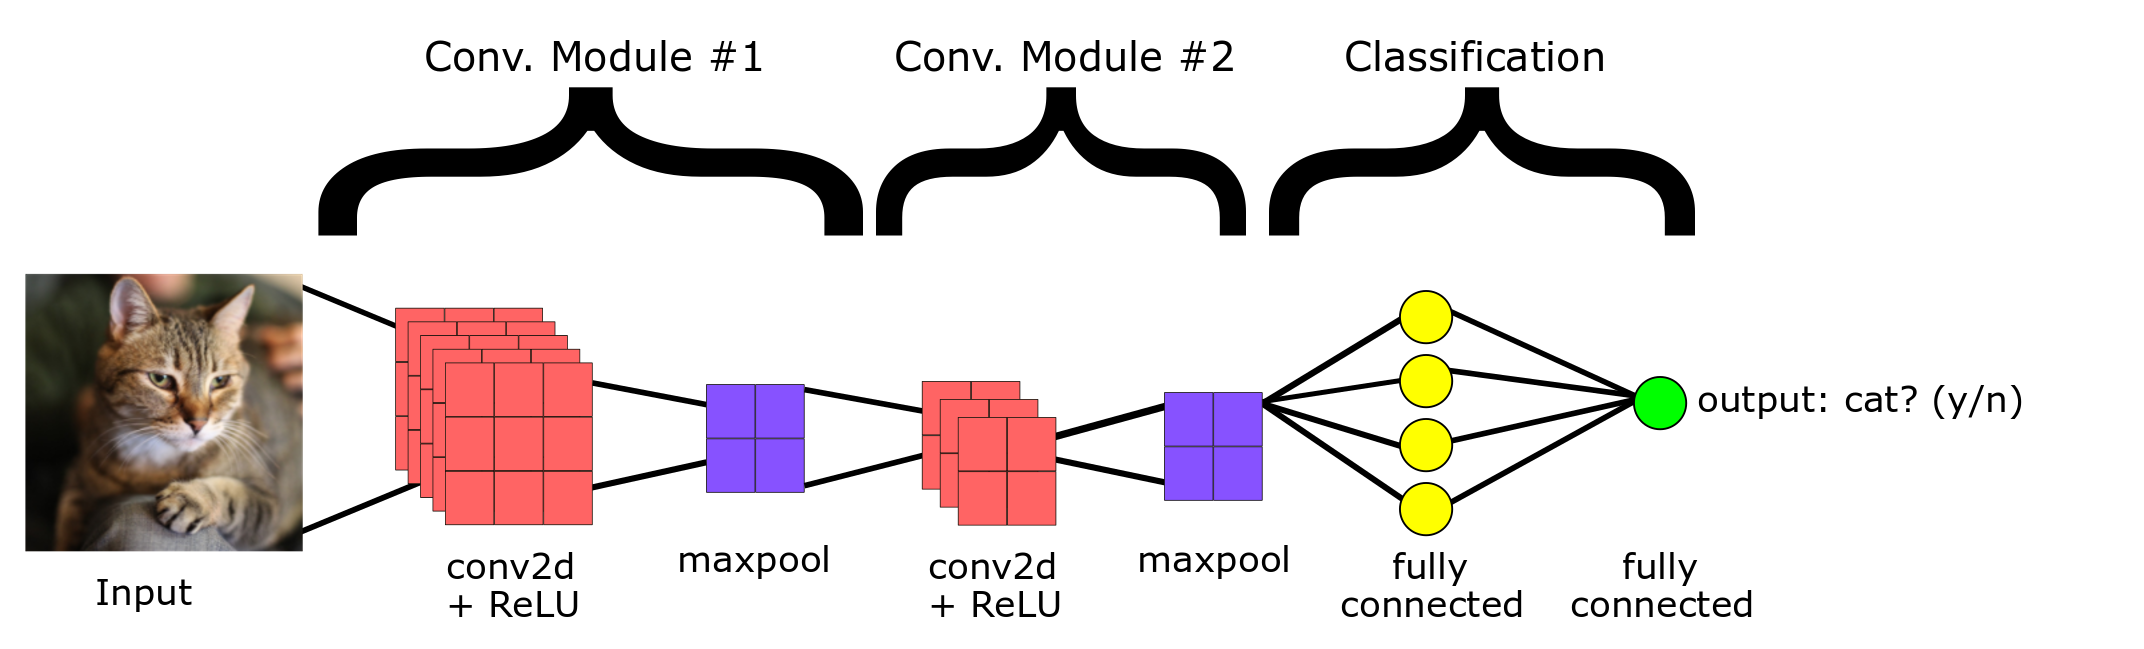
\includegraphics[width=1.1\textwidth]{images/cnn_architecture.png}
\begin{itemize}
\item The CNN shown above contains two convolution modules (convolution + ReLU + pooling) for feature extraction, and two fully connected layers for classification.
\item You often have to experiment to figure out the configuration that produces the best results for their model.
\end{itemize}
\end{frame}

\begin{frame}{Convolution}
\begin{itemize}
\item A convolution extracts tiles of the input feature map, and applies filters to them to compute new features, producing an output feature map, or convolved feature (which may have a different size and depth than the input feature map). 
\item Convolutions are defined by two parameters:
\begin{itemize}
\item Size of the tiles that are extracted (typically 3x3 or 5x5 pixels).
\item The depth of the output feature map, which corresponds to the number of filters that are applied.
\end{itemize}
\end{itemize}
\end{frame}

\begin{frame}{Convolution}
\begin{itemize}
\item During a convolution, the filters (matrices the same size as the tile size) effectively slide over the input feature map's grid horizontally and vertically, one pixel at a time, extracting each corresponding tile.

{\tiny
\url{https://github.com/schneider128k/machine_learning_course/blob/master/slides/images/convolution_overview.gif}}

\item A 3x3 convolution of depth 1 performed over a 5x5 input feature map, also of depth 1. There are nine possible 3x3 locations to extract tiles from the 5x5 feature map, so this convolution produces a 3x3 output feature map.

\item You can also add padding (blank rows/columns with all-zero values) to each side of the input feature map, producing a 7x7 matrix with 5x5 possible locations to extract a 3x3 tile.
\end{itemize}
\end{frame}

\begin{frame}{Convolution}
\begin{itemize}
\item Consider the following input feature map and the following convolutional filter:

\medskip
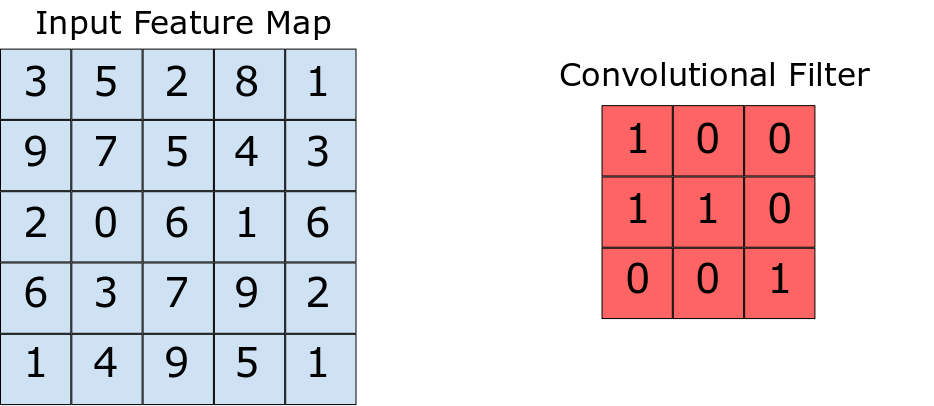
\includegraphics[width=1.0\textwidth]{images/convolution_example.png}
\item Compute the values of the $3\times 3$ output feature map.
\end{itemize}
\end{frame}

\begin{frame}{Convolution}
\begin{itemize}
\item During training, the CNN ``learns'' the optimal values for the filter matrices that enable it to extract meaningful features (textures, edges, shapes) from the input feature map. 
\item As the number of filters (output feature map depth) applied to the input increases, so does the number of features the CNN can extract. 
\item However, the tradeoff is that filters compose the majority of resources expended by the CNN, so training time also increases as more filters are added. 
\item Additionally, each filter added to the network provides less incremental value than the previous one, so we aim to construct networks that use the minimum number of filters needed to extract the features necessary for accurate image classification.
\end{itemize}
\end{frame}

\begin{frame}{ReLU}
\begin{itemize}
\item After each convolution operation, the CNN applies a Rectified Linear Unit (ReLU) transformation to the convolved feature, in order to introduce nonlinearity into the model. 
\item The ReLU function, 
\[
\mathrm{ReLU}(x) = \max(0,x),
\]
returns $x$ for all values of $x > 0$, and returns $0$ for all values of $x \le 0$.
\end{itemize}
\end{frame}

\begin{frame}{Pooling}
\begin{itemize}
\item After ReLU comes a pooling step, in which the CNN downsamples the convolved feature (to save on processing time), reducing the number of dimensions of the feature map, while still preserving the most critical feature information. 
\item A common algorithm used for this process is called max pooling.
\end{itemize}
\end{frame}

%

\begin{frame}{Max pooling}
\begin{itemize}
\item Max pooling operates in a similar fashion to convolution. We slide over the feature map and extract tiles of a specified size. For each tile, the maximum value is output to a new feature map, and all other values are discarded. 
\item Max pooling operations take two parameters:
\begin{itemize}
\item Size of the max-pooling filter (typically 2x2 pixels)
\item Stride: the distance, in pixels, separating each extracted tile. 
\end{itemize}
\end{itemize}
\end{frame}

%

\begin{frame}{Max pooling}
\begin{itemize}
\item Unlike with convolution, where filters slide over the feature map pixel by pixel, in max pooling, the stride determines the locations where each tile is extracted. 
\item For a 2x2 filter, a stride of 2 specifies that the max pooling operation will extract all nonoverlapping 2x2 tiles from the feature map.
\end{itemize}

{\tiny \url{https://github.com/schneider128k/machine_learning_course/blob/master/slides/images/maxpool_animation.gif}}
\end{frame}

%

\begin{frame}{Fully connected layers}
\begin{itemize}
\item At the end of a convolutional neural network are one or more fully connected layers (when two layers are "fully connected," every node in the first layer is connected to every node in the second layer). 
\item Their job is to perform classification based on the features extracted by the convolutions. 
\item Typically, the final fully connected layer contains a softmax activation function, which outputs a probability value from $0$ to $1$ for each of the classification labels the model is trying to predict.
\end{itemize}
\end{frame}

%

\begin{frame}{Key terms}
\begin{itemize}
\item convolutional filter
\item max pooling
\item ReLU
\item stride
\end{itemize}
\end{frame}

\end{document}